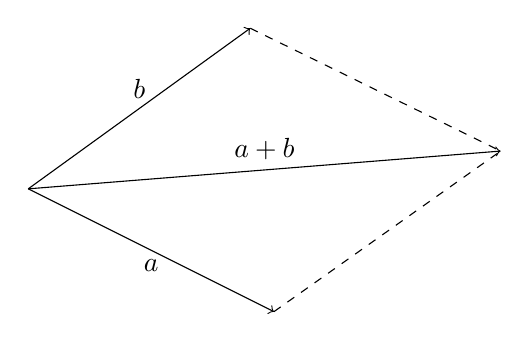
\begin{tikzpicture}[scale=0.6]
\draw[->] (3.6,10.2) -- (8.8,7.6) node[midway, below] {$\ve a$};
\draw[->] (3.6,10.2) -- (8.3,13.6) node[midway, above] {$\ve b$};
\draw[dashed] (8.8,7.6) -- (13.6,11);
\draw[dashed] (8.3,13.6) -- (13.6,11);
\draw[->,black] (3.6,10.2) -- (13.6,11) node[midway, above] {$\ve a + \ve b$};
\end{tikzpicture}
